\chapter{Methodology}
\label{ch:method}

\section{Task formulation}

Dialect identification is posed as 9-way single-label classification: given a
clip of about five seconds, predict one of Barishal, Chattogram, Dhaka, Formal,
Khulna, Mymensingh, Noakhali, Rajshahi or Sylhet. The headline metric is
macro-averaged F1 on the test split, which weights every class equally despite
the imbalance in \cref{tab:classes}; chance level is about 0.11. Every model is
evaluated under the two split protocols of \cref{sec:method-splits}, and every
headline number carries a bootstrap confidence interval
(\cref{sec:method-eval}).

\Cref{fig:pipeline} shows the two routes compared in this thesis. The acoustic
route (\cref{sec:method-acoustic}) classifies the audio directly; the lexical
route (\cref{sec:method-lexical}) transcribes it first and classifies the words.
Both share the splits, the metric and the evaluation code, and their outputs are
combined by late fusion.

\begin{figure}[ht]
  \centering
  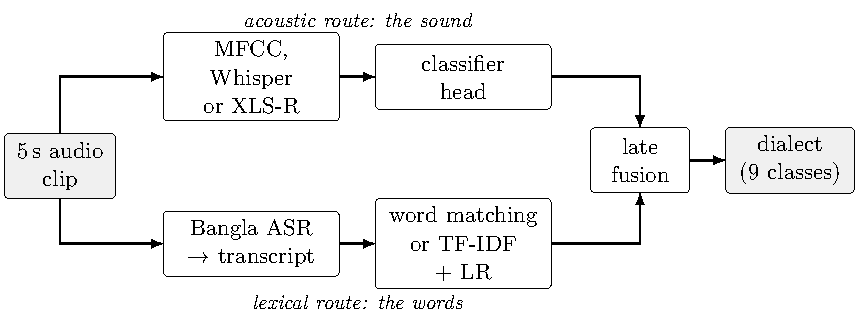
\includegraphics{pipeline}  % source: figures/src/pipeline.tex
  \caption{The two routes to dialect identity. The acoustic route sees only the
  signal; the lexical route sees only the words recovered by speech recognition.
  Each produces class probabilities, which late fusion combines
  (\cref{eq:fusion}).}
  \label{fig:pipeline}
\end{figure}

\section{Splitting protocols}
\label{sec:method-splits}

Two protocols are used throughout (\cref{tab:splits}).

\paragraph{Clip-level split.} \path{build_split.py} draws a stratified
75/10/15 train/validation/test split with seed 42. Clips with a known source
(the 557 sourced Formal clips) are split source-disjointly with
\path{StratifiedGroupKFold}; all other clips are split individually. Because
the same speaker or recording can then appear on both sides, scores under this
protocol are an \emph{upper bound}. The split is committed to the repository
for reproducibility.

\paragraph{Strict pseudo-speaker split.} Each clip is embedded with the
SpeechBrain ECAPA-TDNN speaker model \citep{desplanques2020ecapa}
(\hf{speechbrain/spkrec-ecapa-voxceleb}, 192 dimensions). Within each class the
embeddings are clustered by agglomerative clustering with cosine distance and
average linkage, with no preset number of clusters. The distance threshold is
not hand-picked: it is \emph{calibrated on the Formal class}, whose true sources
are known for 557 clips, by sweeping 0.30--0.90 and keeping the threshold that
maximises the adjusted Rand index \citep{hubert1985ari} between clusters and
true sources. The best threshold is 0.50, with ARI 0.347. Clustering every
class at this threshold yields 1,683 pseudo-speaker groups, and a grouped split
then guarantees that no group crosses train, validation and test (verified: 0
of 1,683).

The modest calibration ARI is acknowledged: pseudo-speakers only partly recover
true sources, so the strict split removes much, but not provably all, of the
speaker and channel overlap. It stands in for true speaker labels, which the
corpus lacks. Formal is not a clean control either: only its 557 sourced clips
are source-disjoint under both protocols, while its other 1,095 clips move from
clip-level splitting to pseudo-speaker grouping like the regional classes.

\begin{table}[ht]
  \centering
  \caption{Split sizes. Per-class test sizes are in \cref{tab:classes}.}
  \label{tab:splits}
  \begin{tabular}{lrrrl}
    \toprule
    Protocol & Train & Validation & Test & Grouping \\
    \midrule
    Clip-level & 6,977 & 997 & 1,329 & sourced Formal clips only \\
    Strict     & 6,931 & 1,045 & 1,327 & 1,683 pseudo-speaker groups \\
    \bottomrule
  \end{tabular}
\end{table}

\section{Acoustic models}
\label{sec:method-acoustic}

All acoustic models share one protocol: inverse-frequency class-weighted
cross-entropy, model selection by validation macro-F1, and seed 42. Models
(a)--(c) are the original comparison; (d) and (e) were added after a
supervisor review, to place Bangla-pretrained encoders beside the multilingual
ones and to fine-tune Whisper as XLS-R was fine-tuned.

\paragraph{(a) MFCC statistics + MLP} (\path{baseline_mfcc.py}). Forty
MFCCs with their first and second differences are mean- and standard-deviation
pooled over time into a 240-dimensional vector, fed to the same head as (b).
This re-implements the spirit of the project's original hand-crafted pipeline
under the current protocol, so that representations are compared fairly.

\paragraph{(b) Frozen Whisper-small + MLP} (\path{baseline_whisper.py}).
Each clip is encoded once by the frozen encoder of \hf{openai/whisper-small};
hidden states are mean-pooled to 768 dimensions and cached. The classifier is a
two-hidden-layer MLP (768--256--256--9, ReLU, dropout 0.3) trained with AdamW
\citep{loshchilov2019adamw} (learning rate $10^{-3}$, weight decay $10^{-4}$)
for 60 full-batch epochs on CPU, which makes it bit-reproducible, keeping the
checkpoint with the best validation macro-F1.

\paragraph{(c) Fine-tuned XLS-R-300M} (\path{finetune_xlsr.py}).
\hf{facebook/wav2vec2-xls-r-300m} with a sequence-classification head; the
convolutional feature encoder is frozen and the Transformer and head are
fine-tuned. Two learning-rate groups (encoder $2\times10^{-5}$, head
$10^{-4}$), 10\,\% linear warm-up then linear decay, batch 8 with gradient
accumulation 2 (effective batch 16), fp16 mixed precision, gradient clipping at
1.0, 20 epochs. Inputs are 5\,s waveforms, padded or trimmed and normalised per
utterance. An 8-epoch pilot (macro-F1 0.865, still rising at the last epoch)
showed that the schedule needed lengthening; at 20 epochs validation plateaus
from about epoch 11 (\cref{fig:training-curve}).

\paragraph{(d) Fine-tuned Whisper-medium encoders} (\path{finetune_xlsr.py --model ...}).
The same recipe as (c), applied to the encoder of three Whisper-medium
checkpoints: \hf{openai/whisper-medium} (multilingual), and the two Bangla
speech-recognition models of \cref{tab:asr-fronts} that share its architecture,
\emph{Tugstugi} (fine-tuned on standard Bangla by Bengali.AI) and \emph{Tugstugi
(Ben-10)} (further fine-tuned on dialect speech). Each is loaded as an
encoder-only classifier: the seq2seq checkpoint's decoder is dropped, and a
projector, mean-pooling over time and a linear classifier are added, mirroring
the XLS-R head (\texttt{WhisperForAudioClassification} in Transformers). Whisper's
encoder is built for 30\,s of input; to train on 5\,s clips at a sixth of the
cost, only the first 250 rows of its (frozen) positional table are kept, which
corresponds to 500 log-mel frames, and the two convolutional input layers are
frozen as XLS-R's feature encoder is. All 24 Transformer layers (302M
parameters) and the head are trained with the hyperparameters of (c), for 12
epochs rather than 20 because XLS-R's validation curve had plateaued by epoch
11 and the larger encoder converges faster; a run takes about 70 minutes on a
T4. Raw amplitude is fed to Whisper's own log-mel front end; the per-utterance
normalisation of (c) is not applied.

\paragraph{(e) Fine-tuned FastConformer} (\path{finetune_xlsr.py --family nemo}).
Hishab's Bangla FastConformer (\hf{hishab/hishab_bn_fastconformer}, NVIDIA NeMo)
is the Bangla-pretrained counterpart of (d) from a different architecture. Its
mel front end and Conformer encoder are taken from the released ASR model, the
encoder output is mean-pooled over the unpadded frames and a linear classifier
is added. The encoder and head are trained with the hyperparameters of (c) for
20 epochs; the encoder is much smaller than Whisper-medium's.

\paragraph{Frozen rows for (d)} (\path{baseline_whisper.py cache --model ...}).
To separate the effect of fine-tuning from that of the encoder, the frozen
recipe of (b) is also run on the Whisper-medium and Tugstugi (Ben-10)
encoders, so that the same checkpoint appears both frozen and fine-tuned.

\paragraph{Augmentation variant} (\path{finetune_xlsr.py --augment}). A
train-only waveform augmentation chain aimed at recording-channel signatures:
gain $\pm 6$\,dB ($p=0.5$), Gaussian noise at 10--30\,dB SNR ($p=0.5$),
seven-band parametric equalisation $\pm 6$\,dB ($p=0.3$), telephone-style
band-pass 300--3400\,Hz ($p=0.15$), pitch shift $\pm 2$ semitones ($p=0.25$),
and time stretch 0.9--1.1 ($p=0.25$).

\section{Evaluation and statistical uncertainty}
\label{sec:method-eval}

Every headline number is one seed on one test set. To separate signal from
sampling noise, \path{bootstrap_ci.py} resamples the saved test predictions
$B = 2{,}000$ times in two ways: resampling clips, and resampling whole
pseudo-speaker or source groups. The group bootstrap is the honest choice,
because clips of one speaker are correlated and a clip bootstrap understates
the variance \citep{efron1993bootstrap}. For each model it reports the 95\,\%
percentile interval of macro-F1, and for each pair of models the interval of
the difference and the proportion of resamples in which the difference is zero
or negative. The clip-level test set contains 565 groups and the strict test
set 230.

\section{Data-efficiency protocol}
\label{sec:method-efficiency}

\path{data_efficiency.py} retrains the MLP head of (a) and (b) on stratified
fractions of 10, 25, 50, 75 and 100\,\% of the training split, three seeds per
point, under both protocols; evaluation is always on the full, fixed test split.
Fine-tuning is excluded because each point would cost a full GPU run.

\section{The lexical route}
\label{sec:method-lexical}

The acoustic models never observe \emph{what} is said. The lexical route asks
how much dialect identity is recoverable from the words alone and whether it
adds to the acoustics. It reuses the splits, the metric and the bootstrap
unchanged, so every number is directly comparable with
\cref{sec:method-acoustic}.

\subsection{Transcription}

The corpus has no transcripts, so text is produced by off-the-shelf Bangla
speech recognition (\path{transcribe.py}). The recognisers follow the Ben-10
benchmark \citep{dipto2025ben10} as far as public checkpoints allow
(\cref{tab:asr-fronts}). \textbf{None was trained or fine-tuned in this work};
each is used as released. Google's paid recogniser and the benchmark's
Ben-10-fine-tuned wav2vec~2.0, which has no public checkpoint, are omitted.

\begin{table}[ht]
  \centering
  \caption{Speech-recognition front-ends. ``Training data'' is as stated by
  the publishers.}
  \label{tab:asr-fronts}
  \small
  \begin{tabularx}{\textwidth}{@{}lL>{\raggedright\arraybackslash}p{3.3cm}@{}}
    \toprule
    Front-end & Checkpoint & Training data \\
    \midrule
    Tugstugi (Ben-10) & \hf{bengaliAI/tugstugi_bengaliai-regional-asr_whisper-medium} & OOD-Speech, then Ben-10 dialect speech \\
    Tugstugi & \hf{bengaliAI/tugstugi_bengaliai-asr_whisper-medium} & OOD-Speech (standard Bangla) \\
    Hishab FastConformer & \hf{hishab/hishab_bn_fastconformer} & $\approx$18k\,h, mostly news \\
    wav2vec2 Bengali\textsuperscript{*} & \hf{arijitx/wav2vec2-xls-r-300m-bengali} & standard Bangla \\
    Whisper-large-v3 & \hf{openai/whisper-large-v3} & multilingual web audio (zero-shot) \\
    \bottomrule
    \multicolumn{3}{@{}l}{\footnotesize\textsuperscript{*}Stand-in for the benchmark's ``Wav2Vec2 (SCB)'', whose checkpoint is not public.}
  \end{tabularx}
\end{table}

Decoding is greedy throughout. For the Whisper models, the language and task
are fixed to Bangla transcription with no prompt and a cap of 128 new tokens on
the 5\,s thesis clips (median output 53 tokens; 0.2\,\% of clips reach 120) and
440 on Ben-10's up-to-30\,s clips; the
two Tugstugi checkpoints ship without a language-token table, so the generation
configuration of the base \hf{openai/whisper-medium} is substituted, which
changes no weights. The wav2vec~2.0 model is decoded by CTC argmax
\citep{graves2006ctc} without a language model; the FastConformer is run through
NVIDIA NeMo \citep{kuchaiev2019nemo}. All 9,303 clips were transcribed on a
Kaggle T4 GPU (43, 45, 82, 15 and 7 minutes for the five front-ends in the
order of \cref{tab:asr-fronts}). A 450-clip pilot run on an Apple M1 agreed with
the T4 output on 93.6\,\% of clips; all reported numbers use the T4
transcripts.

\subsection{Normalisation and the standard-Bangla vocabulary}

All text---transcripts, reference corpora and word lists---passes one tokeniser
(\path{text_utils.py}): Unicode NFC normalisation, Bangla-letter tokens only
(digits, punctuation and Latin script are dropped), word-level normalisation with
\path{bnunicodenormalizer}, and removal of zero-width joiners.

The \emph{standard vocabulary} $V$ is the word inventory of OOD-Speech's
963,636 training sentences \citep{rakib2023oodspeech}: 8.19 million tokens and
156,643 word types, of which the 88,262 types occurring at least three times are
kept to exclude typos. A transcript word outside $V$ is a \emph{candidate
regional word}. The Ben-10 paper characterises its districts by the same
out-of-vocabulary construction.

\subsection{Regional lexicons}

A lexicon maps each region $r$ to a set of words $w$ with a weight
$p(r \mid w)$. With $c_r(w)$ the count of $w$ in region $r$'s text, $N_r$ the
total number of tokens in that text, and add-$\tfrac12$ smoothing,
\begin{equation}
  p(r \mid w) = \frac{(c_r(w) + \tfrac12)/N_r}{\sum_{q} (c_q(w) + \tfrac12)/N_q},
  \label{eq:lexicon-weight}
\end{equation}
so that a word shared by several dialects counts less towards each. Two
lexicons are built (\path{build_lexicon.py}):
\begin{itemize}
  \item The \textbf{external lexicon} comes from human-written dialect text
        independent of the corpus: the Ben-10 training transcripts and the
        regional side of Vashantor (\cref{sec:data-external}). A Vashantor word
        that also appears on the standard side of the same sentence pair is not
        counted as regional. Districts are matched by exact name only, so the
        external lexicon covers Barishal, Chattogram, Sylhet, Noakhali and
        Mymensingh.
  \item The \textbf{in-domain lexicon} comes from the speech-recognition
        transcripts of the \emph{training split only}---verified in code: no
        validation or test clip contributes. A candidate regional word is kept
        for a class if it occurs at least three times across at least two
        pseudo-speakers of that class, which suppresses recognition noise and
        programme-specific words. It covers all classes and is built separately
        for each front-end and each split protocol.
\end{itemize}

\subsection{Classifiers}

Three classifiers operate on the transcripts (\path{lexical_did.py}).

\paragraph{Word matching.} For a clip with tokens $t_1, \dots, t_n$, the
\emph{non-formal share} is $f = \frac{1}{n}\sum_i \mathbb{1}[t_i \notin V]$, and
the \emph{match percentage} for each region is
\begin{equation}
  s_r = \frac{1}{n} \sum_{i=1}^{n} p(r \mid t_i),
  \label{eq:match}
\end{equation}
where $p(r \mid t_i) = 0$ for words absent from region $r$'s lexicon. A clip
with $f < \tau$, or with $s_r = 0$ for every region, is classified as Formal;
otherwise it is assigned to $\arg\max_r s_r$. The threshold $\tau$ is chosen on
the validation split. The method needs no training, and the per-word evidence
behind each decision can be shown to a user.

\paragraph{TF-IDF + logistic regression.} The normalised transcript is
represented by TF-IDF features over word 1--2-grams and character 2--5-grams
(sublinear term frequency, minimum document frequency 2), and classified by
logistic regression with balanced class weights, with the regularisation
strength $C \in \{0.3, 1, 3, 10, 30\}$ chosen on validation
\citep{pedregosa2011sklearn}. Unlike word matching, it uses standard words too.

\paragraph{Late fusion.} With $p_\text{a}$ the class probabilities of the
fine-tuned XLS-R model and $p_\text{l}$ those of the TF-IDF model,
\begin{equation}
  \hat{y} = \arg\max_{c}\; \alpha \log p_\text{a}(c) + (1 - \alpha) \log p_\text{l}(c),
  \label{eq:fusion}
\end{equation}
with $\alpha \in \{0, 0.05, \dots, 1\}$ chosen on validation. XLS-R
probabilities are computed from the Phase~2 and Phase~3 checkpoints on the same
5\,s inputs used in training; their arg\,max reproduces the saved test
predictions exactly on the strict split and on 1,328 of 1,329 clip-level clips,
the one difference coming from M1 versus T4 arithmetic.

\subsection{Speech-recognition reference evaluation}
\label{sec:method-ben10}

The corpus has no reference transcripts, so recognition quality is measured on
Ben-10's public validation set (1,666 clips from ten districts,
\path{ben10_eval.py}). Besides corpus-level word and character error rates on
normalised tokens \citep{jiwer}, \emph{dialect-word recall} is the proportion of
reference tokens outside $V$ that the hypothesis reproduces exactly (counts
matched per clip). It is the full-set, automated counterpart of the Ben-10
paper's hand-counted dialect recall over about 50 words per district.
\emph{Formal-word recall} is the same measure for reference tokens inside $V$.
On the corpus itself, which has no references, the share of transcript tokens
outside $V$ per class is reported for each front-end.

\section{Compute and reproducibility}

Development and all experiments except fine-tuning and transcription ran on an
Apple M1 laptop (16\,GB, PyTorch MPS backend). Fine-tuning ran on Kaggle's free
T4 GPU tier: about 2.5 hours per XLS-R run, 55--75 minutes per Phase 6 run
(about 9 hours for the eight), and about 4.5 hours in all for the lexical
route's transcription. The pipeline survived a mid-project hardware change (GTX 1660 Ti to
M1) with the frozen-embedding baseline reproducing within 0.3 macro-F1 points.
The code uses PyTorch \citep{paszke2019pytorch}, Hugging Face Transformers
\citep{wolf2020transformers}, SpeechBrain \citep{ravanelli2021speechbrain},
librosa \citep{mcfee2015librosa} and scikit-learn \citep{pedregosa2011sklearn}.
\Cref{app:repro} maps every reported number to the command that produces it.
